\documentclass[11pt,a4paper]{article}

% =========================================================
% CONFIGURACIÓN GENERAL
% =========================================================

\usepackage[a4paper,margin=2.5cm]{geometry}

% --- Idioma y codificación ---
\usepackage[utf8]{inputenc}
\usepackage[T1]{fontenc}
\usepackage[spanish,es-tabla]{babel}

% --- Tipografía ---
\usepackage{helvet}
\renewcommand{\familydefault}{\sfdefault}

% --- Elementos gráficos y formato ---
\usepackage{graphicx}
\usepackage{xcolor}
\usepackage{enumitem}
\usepackage{booktabs}
\usepackage{microtype}
\usepackage{titlesec}
\usepackage{fancyhdr}
\usepackage{setspace}
\usepackage{caption}
\usepackage{tikz}

% --- Enlaces ---
\usepackage[
    colorlinks=true,
    linkcolor=uamorange,
    urlcolor=uamorange,
    citecolor=uamorange
]{hyperref}

% =========================================================
% COLORES
% =========================================================

% Naranja institucional de la UAM, utilizado de forma discreta
\definecolor{uamorange}{HTML}{E85F24}

% Tonos neutros para una apariencia académica
\definecolor{darkgray}{HTML}{333333}
\definecolor{mediumgray}{HTML}{666666}
\definecolor{lightgray}{HTML}{EAEAEA}

% =========================================================
% CONFIGURACIÓN DE SECCIONES
% =========================================================

\titleformat{\section}
    {\Large\bfseries\color{darkgray}}
    {\thesection.}
    {0.6em}
    {}
    [\vspace{0.25em}\color{uamorange}\rule{\textwidth}{0.8pt}]

\titleformat{\subsection}
    {\large\bfseries\color{darkgray}}
    {\thesubsection}
    {0.6em}
    {}

\titleformat{\subsubsection}
    {\normalsize\bfseries\color{darkgray}}
    {\thesubsubsection}
    {0.6em}
    {}

\titlespacing*{\section}
    {0pt}{2.2em}{1.2em}

\titlespacing*{\subsection}
    {0pt}{1.5em}{0.7em}

\titlespacing*{\subsubsection}
    {0pt}{1.2em}{0.5em}

% =========================================================
% ENCABEZADO Y PIE DE PÁGINA
% =========================================================

\pagestyle{fancy}
\fancyhf{}

\fancyhead[L]{\small\textcolor{mediumgray}{Plataforma de Distribución de Videojuegos}}
\fancyhead[R]{\small\textcolor{mediumgray}{Modelo Relacional}}

\fancyfoot[C]{%
    \small\textcolor{mediumgray}{Universidad Autónoma Metropolitana --- Unidad Cuajimalpa}
    \hspace{0.5em}
    \textcolor{uamorange}{\textbullet}
    \hspace{0.5em}
    \thepage
}

\renewcommand{\headrulewidth}{0.4pt}
\renewcommand{\footrulewidth}{0pt}

\setlength{\headheight}{14pt}

% =========================================================
% LISTAS
% =========================================================

\setlist[itemize]{
    leftmargin=1.8em,
    itemsep=0.35em,
    topsep=0.5em
}

\setlist[enumerate]{
    leftmargin=2em,
    itemsep=0.5em,
    topsep=0.5em
}

% =========================================================
% FIGURAS
% =========================================================

\captionsetup{
    font=small,
    labelfont=bf,
    labelsep=period,
    justification=centering
}

% =========================================================
% INTERLINEADO
% =========================================================

\setstretch{1.12}

% =========================================================
% DOCUMENTO
% =========================================================

\begin{document}

% =========================================================
% PORTADA
% =========================================================

\begin{titlepage}
\thispagestyle{empty}

\centering

\vspace*{1.2cm}

% Logo institucional
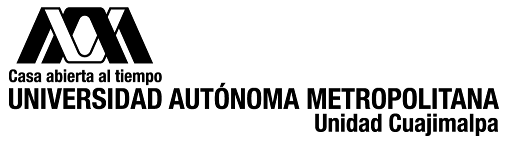
\includegraphics[width=0.38\textwidth]{imagenes/uam_logo.png}

\vspace{1.4cm}

{\large
\textbf{UNIVERSIDAD AUTÓNOMA METROPOLITANA}
\par}

\vspace{0.25cm}

{\normalsize
Unidad Cuajimalpa
\par}

\vspace{0.9cm}

% Línea decorativa discreta
{\color{uamorange}\rule{0.55\textwidth}{1.2pt}}

\vspace{1.1cm}

{\large
\textbf{Laboratorio Temático III}
\par}

\vspace{2.2cm}

{\Huge
\bfseries
Documentación del\\[0.15cm]
Modelo Relacional
\par}

\vspace{0.7cm}

{\Large
\textcolor{uamorange}{
Plataforma de Distribución de Videojuegos
}
\par}

\vspace{2.8cm}

{\large\textbf{Autores}}
\par

\vspace{0.6cm}

{\large Ramos Reyes Aaron Rodrigo\par}
\vspace{0.25cm}
{\large Cruz Lopez Ana Lilia Guadalupe\par}
\vspace{0.25cm}
{\large Alan Reyes Rosales\par}

\vfill

{\normalsize
\today
\par}

\end{titlepage}

% =========================================================
% CONTENIDO
% =========================================================

\section{Introducción}

El presente proyecto consiste en el diseño e implementación de una base de datos relacional para una plataforma de distribución digital de videojuegos y software, inspirada en el modelo de negocio y funcionalidades de Steam. El objetivo principal es proveer una estructura robusta, escalable y libre de anomalías que permita gestionar el ciclo de vida completo del usuario en la plataforma: desde su registro e interacción social, hasta la exploración del catálogo, el procesamiento de compras y la gestión de su biblioteca personal de títulos. Esta arquitectura de datos servirá como la capa de persistencia para una futura API REST.

\section{Flujo de Uso del Sistema}

El diseño de la base de datos soporta de forma nativa el siguiente flujo de interacción del usuario:

\begin{enumerate}[label=\arabic*.]
\item \textbf{Autenticación e Identidad:} El visitante se registra creando un \texttt{Usuario}. A partir de ese momento, puede establecer conexiones sociales agregando a otros usuarios a su lista de \texttt{Amigos}.

\item \textbf{Exploración del Catálogo:} El usuario navega por los \texttt{Productos} disponibles, los cuales están clasificados por múltiples \texttt{Categorías} y asociados a un \texttt{Desarrollador}.

\item \textbf{Intención de Compra:} Si un usuario tiene interés en un producto, puede añadirlo a su lista de \texttt{Deseados} para un seguimiento a futuro, o agregarlo al \texttt{Carrito} especificando las cantidades.

\item \textbf{Proceso de Checkout:} El sistema consolida los elementos del carrito en una \texttt{Orden} de compra, desglosando los elementos en el \texttt{Detalle\_de\_Orden}.

\item \textbf{Transacción:} Se genera una \texttt{Transacción} vinculada a un \texttt{Método\_de\_Pago} (ej. Tarjeta de Crédito, PayPal). Si la transacción es aprobada, el flujo avanza.

\item \textbf{Aprovisionamiento:} Los productos adquiridos se transfieren a la \texttt{Biblioteca} del usuario de forma permanente.

\item \textbf{Interacción Post-Compra:} Una vez en su biblioteca, el usuario acumula horas de juego y puede redactar \texttt{Reseñas} públicas, recomendando o no el producto.
\end{enumerate}

\section{Explicación de las Tablas y sus Relaciones}

Para que el sistema funcione sin errores, la información no se guarda toda junta, sino que se divide en distintas tablas que se conectan entre sí. A continuación, explicamos cada relación de forma sencilla:

\subsection{Catálogos y Entidades Base}

\begin{itemize}
\item \textbf{Usuario:} Guarda la información de las personas registradas (correo, contraseña, teléfono).

\item \textbf{Producto:} Guarda los detalles básicos de los videojuegos (nombre, precio, imagen).

\item \textbf{Desarrollador y Categoría:} Son listas independientes que nos ayudan a clasificar los juegos sin escribir los nombres a mano cada vez, evitando errores de dedo.

\item \textbf{Método de Pago:} Lista con las opciones habilitadas para pagar (tarjeta, PayPal, transferencias, etc.).
\end{itemize}

\subsection{¿Cómo se relacionan los Usuarios con los Productos?}

Como un usuario interactúa con los juegos de muchas maneras, usamos tablas intermedias para conectar la tabla \textbf{Usuario} con la tabla \textbf{Producto}:

\begin{itemize}
\item \textbf{Biblioteca (Muchos a Muchos):} Un usuario compra muchos juegos, y un juego es adquirido por muchos usuarios. Esta tabla los une y guarda el precio exacto que el usuario pagó y la fecha en que lo consiguió.

\item \textbf{Carrito (Muchos a Muchos):} Funciona como la canasta del supermercado. Conecta al usuario con los juegos que está a punto de comprar, guardando también cuántas copias (cantidad) quiere de cada uno.

\item \textbf{Deseados (Muchos a Muchos):} Es la lista de deseos. Conecta al usuario con los juegos que le interesan para el futuro, guardando la fecha en que los agregó.

\item \textbf{Reseñas (Muchos a Muchos):} Un usuario puede opinar sobre varios juegos, y un juego recibe opiniones de muchos usuarios. Aquí guardamos su comentario, si lo recomienda o no, y cuántas horas ha jugado.
\end{itemize}

\subsection{Otras Relaciones Importantes}

\begin{itemize}
\item \textbf{Amigos (Usuario con Usuario):} Un usuario puede tener muchos amigos en la plataforma. Usamos esta tabla para conectar a un Usuario con otro Usuario y guardar la fecha en la que se conectaron.

\item \textbf{Producto - Desarrollador (Muchos a Uno):} Un estudio creador (como Epic Games o Valve) hace muchos juegos. Cada juego se conecta a su creador a través del ID del desarrollador.

\item \textbf{Producto - Categoría (Muchos a Muchos):} Un juego puede ser de ``Aventura'' y ``Acción'' al mismo tiempo, y la categoría ``Aventura'' abarca muchos juegos. La tabla \texttt{Producto\_Categoria} se encarga de hacer estos múltiples enlaces.
\end{itemize}

\subsection{El Proceso de Compra (Órdenes y Transacciones)}

Para llevar un control financiero exacto, las ventas se estructuraron de esta manera:

\begin{itemize}
\item \textbf{Usuario - Orden (Uno a Muchos):} Un usuario puede hacer muchas compras a lo largo del tiempo. Cada compra genera un ``ticket'' general llamado \texttt{Orden}.

\item \textbf{Orden - Detalle de Orden (Uno a Muchos):} La \texttt{Orden} es el total a pagar, pero el \texttt{Detalle\_de\_Orden} son los ``renglones'' de ese ticket.

\item \textbf{Producto - Detalle de Orden (Uno a Muchos):} Cada ``renglón'' del ticket se conecta directamente con un \texttt{Producto} para saber exactamente qué juego se vendió en esa compra y a qué precio unitario.

\item \textbf{Orden - Transacción (Uno a Muchos):} Para pagar una Orden, se hace un intento de cobro llamado \texttt{Transacción}. Aquí anotamos si el cobro fue ``Aprobado'', ``Rechazado'' o ``Reembolsado''.

\item \textbf{Transacción - Método de Pago (Muchos a Uno):} Cada intento de cobro se enlaza a un método de pago de nuestro catálogo para saber si el cliente usó tarjeta, saldo de cartera, etc.
\end{itemize}

\section{¿Por qué se organizó así? (Reglas de Normalización)}

El diseño de esta base de datos sigue reglas profesionales para evitar que la información se duplique, se vuelva contradictoria o se pierda. En una presentación, esto significa:

\begin{itemize}
\item \textbf{Cada dato en su lugar (1NF):} Evitamos meter mucha información mezclada en un solo espacio. Por ejemplo, en lugar de escribir un párrafo revuelto con los requisitos de la computadora (memoria, procesador), usamos un formato estructurado (\texttt{JSON}) para que el sistema lo lea fácilmente.

\item \textbf{Dependencia directa (2NF):} En las tablas que unen dos elementos (como un Usuario y un Producto en el Carrito), los datos adicionales como la ``Cantidad'' dependen exclusivamente de ese cruce en particular, no del usuario por separado ni del juego por separado.

\item \textbf{Evitar la repetición de datos (3NF):} Si guardáramos el nombre del creador (\textit{Desarrollador}) directamente dentro del juego y ese estudio cambiara de nombre, tendríamos que buscar y actualizar miles de juegos uno por uno. Al separar al desarrollador en su propia tabla, solo modificamos el nombre una vez y todos sus juegos se actualizan en cascada de forma automática.
\end{itemize}

% =========================================================
% DIAGRAMA
% =========================================================

\newpage

\section{Diagrama de la Base de Datos}

A continuación se presenta el Modelo Entidad-Relación (EER) generado a partir de la implementación en MySQL, el cual ilustra de manera visual todas las tablas, atributos y las conexiones descritas a lo largo de este documento.

\vspace{0.8cm}

\begin{figure}[ht]
\centering

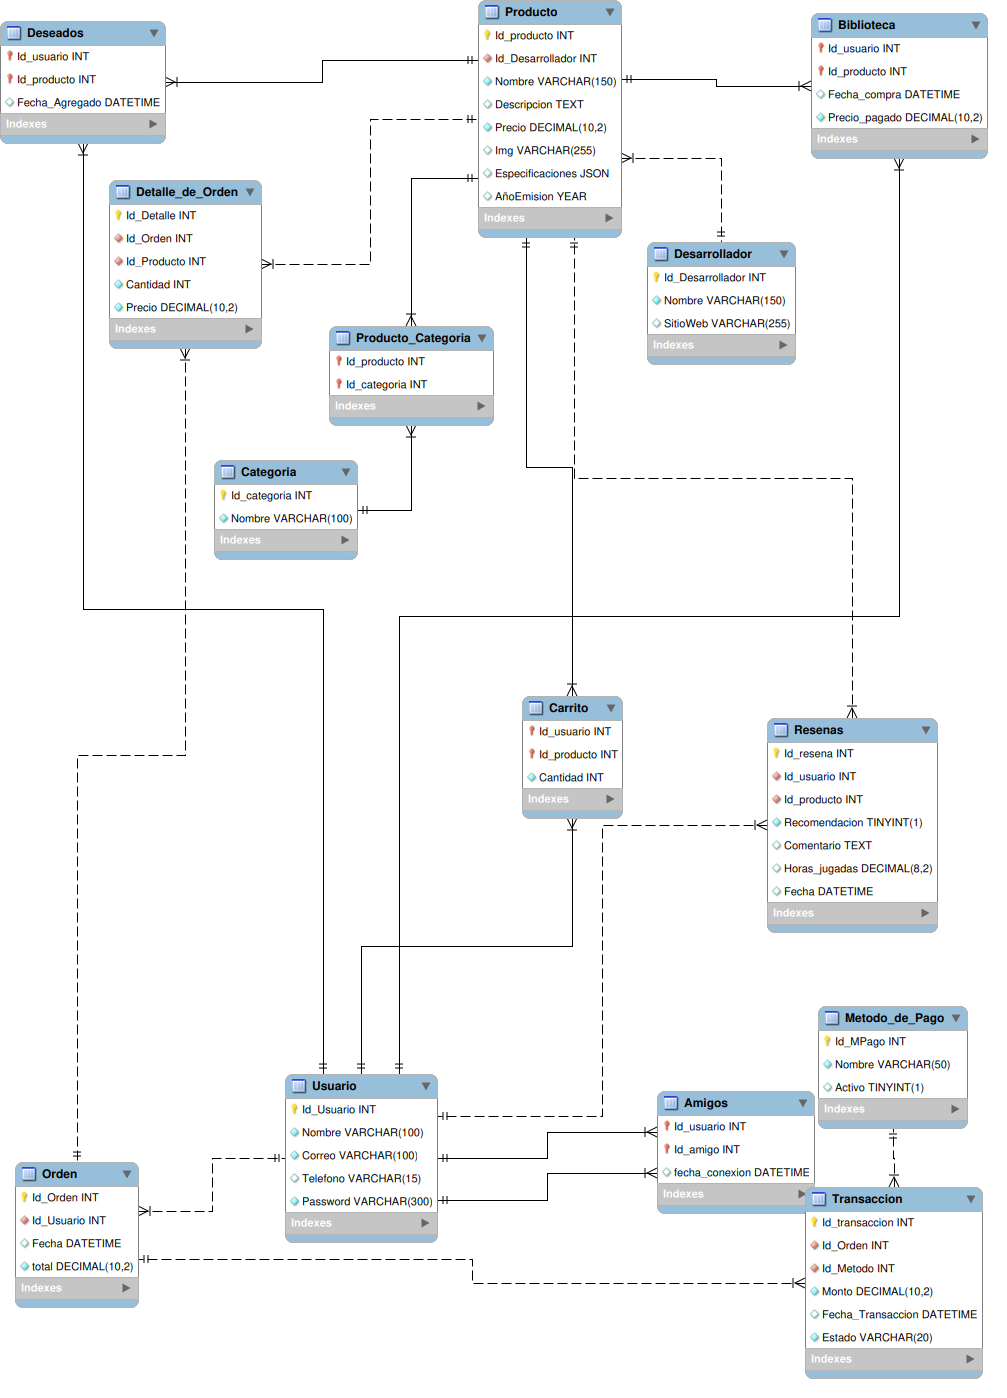
\includegraphics[
    width=\textwidth,
    height=0.72\textheight,
    keepaspectratio
]{imagenes/Diagrama_entidad_relacion.png}

\caption{Modelo Entidad-Relación de la Plataforma}

\end{figure}

\end{document}
```
